\chapter{Time-Domain} \label{cha:time_domain}

In \charef{cha:discretization_schemes}, we have discussed about the
discretization in space of Maxwell equations, for an unstructured
grid. The time-domain version of Maxwell equations, though, present a
derivatives in time that have to be discretized as well. Luckily
enough, being time one-dimensional, the discretization scheme can only
be collocated or uncollocated, i.e. with all the physical quantities
associated to the same time or with a time grid for each of them, as
described in \secref{sec:geometry_and_physics}.

For the reasons that will be explained in \secref{sec:stability_time},
we have chosen, for our algorithm, an uncollocated scheme, already
widely used in electromagnetic simulation software, like the \FDTD: the
\emph{leapfrog timestepping}\index{Leapfrog timestepping}.

\section{Leapfrog Timestepping} \index{Leapfrog timestepping|(} \label{sec:leapfrog}

In \cite{taflove_computational} a precise description of the leapfrog
timestepping, applied to a Cartesian grid\index{Cartesian grid}, is given. Applying it to
our unstructured grid is not different \cite{bolla_piers}.

A more detailed description of the method is given in
\secref{sec:stability_time}, but it's worth seeing now how it applies to
our algorithm.

Let's divide the time in discrete points, or instants, $t_0, t_1, \dotsc, t_n$:
this automatically identifies time intervals
$[t_0,t_1],[t_1,t_2],\dotsc,[t_{n-1},t_n]$. Dual instants
$\Dual{t_0},\Dual{t_1},\dotsc,\Dual{t_n}$ are chosen
at the midpoints of primal intervals (\figref{fig:timeline}).

\begin{figure}[htbp]
  \begin{center}
    \resizebox{8cm}{!}{\input{pics/timeline.pdf_t}}
  \end{center}
  \caption{Discretization of time: dual instants (in blue) are the
    midpoints of primal intervals.}  
  \label{fig:timeline}
\end{figure}

We arbitrarily associate the electric field $\E$ to primal instants;
the Faraday equation in \eqref{eqn:maxwell_integral} tells us to
associate the partial derivative $\partial_t \B$ to the same primal
instants. Using a central difference scheme to discretize the
derivative in time at the first order, we have:
\begin{equation*}
\dt \Evaluate{\B}{t_n} = \frac{\Evaluate{\B}{t_{n+1/2}} -
\Evaluate{\B}{t_{n-1/2}}}{t_{n+1/2}-t_{n-1/2}}.
\end{equation*}

$\B$ is evaluated at timesteps $t_{-1/2}, t_{1/2}, \dotsc, t_{n-1/2}$,
$t_{n+1/2}$, i.e. on dual instants.

A word about notation: from now on, the value of a field $\Vector{F}$
evaluated at the timestep $t_n$ is written as:
\begin{equation*}
  \Evaluate{\Vector{F}}{t_n} = \Disc{\Vector{F}}{}{n}.
\end{equation*}

\index{Leapfrog timestepping|)}

\section{Sources}

Before being able to write the complete set of the discretized Maxwell
equations in the time-domain, we need to implement sources.

There are many possible sources of an electromagnetic field: in our
algorithm, we have implemented two \cite{bolla_piers}.
\begin{description}
\item[Current sources]: they are used to model antennas and
  dipoles. They are very easy to model, because they are already in
  Maxwell equations, identified by the electric current $\J$ and
  magnetic current $\M$.
\item[Field sources]: they are used if the electromagnetic field
  distribution is known on a surface inside or on the boundary of the
  domain\footnote{Strictly speaking, just the tangential part of the
  electromagnetic field is sufficient}. This is a very common
  situation: one of the most interesting problems is to study the
  behavior of a device whose input is provided by some modes of an
  input waveguide: in this case, the field distribution is known at
  the input waveguide cross section and we want to compute the field
  inside the device under test. Modeling these sources is not a
  trivial task, though. The \emph{Equivalence Theorem}
  \cite{someda_electromagnetic} helps us. It reads that the
  electromagnetic field inside a region $R$, generated by a field
  distribution ${\E_i,\H_i}$ at its boundary $dR$, is equivalent to
  the one generated by two surface currents $\J_s$ and $\M_s$ on $dR$,
  whose linear densities are given by:
  \begin{align*}
    \J_s = \CrossProd{\Versor{n}}{\H_i} && \M_s = \CrossProd{\E_i}{\Versor{n}} ,
  \end{align*}
  where $\Versor{n}$ is the normal versor to $dR$.
  
  With the choice of degrees of freedom explained in \eqref{eqn:dof}, $\J_s$ and $\M_s$
  are naturally associated with primal and dual surfaces respectively,
  as fluxes through them (see \figref{fig:sources}). Note that we can
  pass from a linear current density to a flux through a surface using
  the Dirac $\delta$ function:
  \begin{equation*}
    J(x,y,z) = J_s(x,y) \delta(z).
  \end{equation*}
  
  \begin{figure}[htbp]
    \begin{center}
      \resizebox{6cm}{!}{\input{pics/source.pdf_t}}
    \end{center}
    \caption{Electric sources are associated to the dual surfaces,
      magnetic sources to the primal surfaces. If the electromagnetic
      field distribution is known on the blue line, we can use the
      \emph{Equivalence Theorem} to build equivalent sources: at
      limit, we can think of the line (in two dimensions) over which
      the equivalent sources are defined as an infinitesimally thin
      surface.}
    \label{fig:sources}
  \end{figure}

  It is as if we thought to reduce the surfaces, through which we are
  computing the fluxes, to segments: the limiting process gives linear
  densities. Finally, in the coordinate system of
  \figref{fig:sources}, we can write:
  \begin{equation*}
    \int_{\tilde{S}}{\DotProd{\J}{\Versor{y}}d\tilde{S}} = 2\DotProd{\CrossProd{\Versor{n}}{\H}}{\Versor{y}}.
  \end{equation*}

  Note that if we only decide to excite one of the $\J_s$ and $\M_s$
  fields, we'll excite two electromagnetic waves, propagating in
  opposite directions. This is accounted for by the factor $2$ in the
  equation above. To have a wave propagating in one direction, we
  need to excite both $\J_s$ and $\M_s$ at the same time. 
\end{description}

\figref{fig:pml_tuning} shows an example of field sources usage: they
have been applied to tune the PMLs and achieve optimal performance (see
\secref{sec:pml} for the description of PMLs). As
long as there is no optimal design parameters for the PMLs, but they
depend on the particular domain \cite{taflove_computational}, we have
studied a problem whose solution is known analytically: a simple
dielectric slab waveguide.

\begin{figure}[htbp]
  \begin{center}
    \subfigure[Waveguide.]{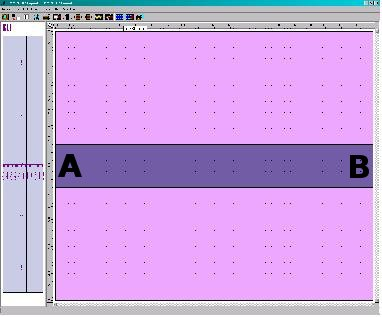
\includegraphics[height=3cm]{pics/source_pml1}}
    \subfigure[Badly tuned PMLs.]{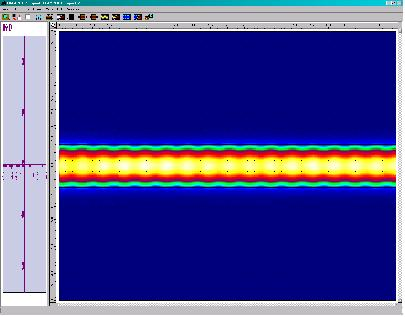
\includegraphics[height=3cm]{pics/source_pml2}}
    \subfigure[Finely tuned PMLs.]{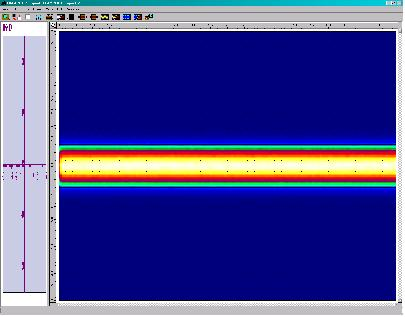
\includegraphics[height=3cm]{pics/source_pml3}}
  \end{center}
  \caption{PMLs tuning by field sources: if finely tuned, PMLs give no
    reflections to the input and output facets of the waveguide.}
  \label{fig:pml_tuning}
\end{figure}  

The input source is provided by the fundamental mode of the waveguide,
computed by FIMMWAVE \cite{fimmwave}: the optimal PMLs
parameters are computed imposing the minimum reflection at the right
hand side facet. To estimate reflections we define the \emph{transmission
coefficient} and the \emph{reflection coefficient} of the device as:
\begin{align*}
  T_j & = \int_B \DotProd{\CrossProd{\E_B}{\Conj{\H_{m_i}}}}{\Versor{x}} dB \\
  R_j & = \int_A
  \DotProd{\CrossProd{(\E_A-\E_{m_i})}{\Conj{\H_{m_i}}}}{\Versor{x}} dA = \int_A
  \DotProd{\CrossProd{\E_A}{\Conj{\H_{m_i}}}}{\Versor{x}} dA - 1,
\end{align*}
where $x$ is the axis of the waveguide, $A$ is the left-hand side
facet of the waveguide, $B$ the right-hand side facet and
$\left\{\E_{m_i},\H_{m_i}\right\}$ is the $m_i$ mode of the waveguide.

We have estimated that we obtain negligible reflections, below $40
dB$, for a PML thickness of about $1 \lambda$ and parabolic losses
profile.

\section{Matricial Representation}

We are now ready to write the complete discretized Maxwell equation in
the time domain \cite{trevisan_geometric}.

Starting from \eqref{eqn:discrete_ampere} and
\eqref{eqn:discrete_faraday}, with the material equations
(\eqref{eqn:discrete_electric} and \eqref{eqn:discrete_magnetic}) and
using the leapfrog timestepping\index{Leapfrog timestepping} to discretize the partial derivative
in time, we obtain:
\begin{equation} \label{eqn:maxwell_time_domain} \begin{cases} 
    \Disc{\Array{d}}{}{n+1} = \Disc{\Array{d}}{}{n} + \deltat
    \Prod{\Transpose{\Matrix{R}}}{\Disc{\Array{h}}{}{n+1/2}} - \Disc{\Array{j}}{}{n+1/2} \\
    \Disc{\Array{e}}{}{n+1} = \Prod{\Matrix{M}_\epsilon}{\Disc{\Array{d}}{}{n+1}} \\
    \Disc{\Array{b}}{}{n+3/2} = \Disc{\Array{b}}{}{n+1/2} - \deltat
    \Prod{\Matrix{R}}{\Disc{\Array{e}}{}{n+1}} + \Disc{\Array{m}}{}{n+1} \\
    \Disc{\Array{h}}{}{n+3/2} = \Prod{\Matrix{M}_\mu}{\Disc{\Array{b}}{}{n+3/2}}
\end{cases} , \end{equation}
where the vectors are defined in \secref{sec:geometry_and_physics} and
the matrices $\Matrix{M}_\epsilon$ and $\Matrix{M}_\mu$ are defined in
\charef{cha:material_equations}. Ohm losses can also be included: see
\secref{sec:ohm_losses}.

The initial conditions are $\Disc{\Array{d}}{}{0}$,
$\Disc{\Array{j}}{}{1/2}$, $\Disc{\Array{h}}{}{1/2}$ and
$\Disc{\Array{m}}{}{1}$: all the other fields, at every timestep,
are \emph{explicitly} computed from these.

We can note that in the simple formulation of
\eqref{eqn:maxwell_time_domain}, the $\Array{e}$ and the $\Array{h}$
vectors are \emph{auxiliary} fields: the constitutive equations are so
easily expressed that they can be included in the Ampere and
Faraday equations:
\begin{equation*} \begin{cases}
    \Disc{\Array{d}}{}{n+1} & = \Disc{\Array{d}}{}{n} + \deltat
    \Prod{\Transpose{\Matrix{R}}}{\Prod{\Matrix{M}_\mu}{\Disc{\Array{b}}{}{n+1/2}}}
    - \Disc{\Array{j}}{}{n} \\
    \Disc{\Array{b}}{}{n+3/2} & = \Disc{\Array{b}}{}{n+1/2} - \deltat
    \Prod{\Matrix{R}}{\Prod{\Matrix{M}_\epsilon}{\Disc{\Array{d}}{}{n+1}}}
    + \Disc{\Array{m}}{}{n+1/2}
  \end{cases} \end{equation*}
or, viceversa, we can consider $\Array{d}$ and $\Array{b}$ auxiliary
and write:
\begin{equation} \label{eqn:maxwell_time_domain_reduced} \begin{cases}
    \Disc{\Array{e}}{}{n+1} & = \Disc{\Array{e}}{}{n} + \deltat
    \Prod{\Matrix{M}_\epsilon}{\Prod{\Transpose{\Matrix{R}}}{\Disc{\Array{h}}{}{n+1/2}}}
    - \Prod{\Matrix{M}_\epsilon}{\Disc{\Array{j}}{}{n}} \\
    \Disc{\Array{h}}{}{n+3/2} & = \Disc{\Array{h}}{}{n+1/2} - \deltat
    \Prod{\Matrix{M}_\mu}{\Prod{\Matrix{R}}{\Disc{\Array{e}}{}{n+1}}}
    + \Prod{\Matrix{M}_\mu}{\Disc{\Array{m}}{}{n+1/2}}
\end{cases} . \end{equation}

We can further simplify Maxwell equations obtaining the discrete
Helmholtz equation. Derive in time \eqref{eqn:discrete_ampere} and
substitute it in \eqref{eqn:discrete_faraday}, using
\eqref{eqn:discrete_magnetic} and \eqref{eqn:discrete_electric}. We
obtain:
\begin{equation} \label{eqn:discrete_helmholtz}
  \Prod{\Prod{\Matrix{M}_\epsilon}{\Prod{\Transpose{\Matrix{R}}}{\Prod{\Matrix{M}_\mu}{\Matrix{R}}}}}{\Array{e}}
  = -\partial_t^2 \Array{e} .
\end{equation}

With the leapfrog timestepping, this scheme is stable only if the
eigenvalues of the matrix $\Matrix{A} =
\Prod{\Matrix{M}_\epsilon}{\Prod{\Transpose{\Matrix{R}}}{\Prod{\Matrix{M}_\mu}{\Matrix{R}}}}$
are real and positive \cite{liu_fourier}. As we'll show later, a
sufficient condition is that the material matrices
$\Matrix{M}_\epsilon$ and $\Matrix{M}_\mu$ are symmetric and positive
definite \cite{schuhmann_whitney,schuhmann_stability}. This condition
is easily satisfied for Vorono\"i grids, where the material matrices
are diagonal, but special care must be taken for other kinds of dual
grids.

\section{Stability of Time Discretization}
\index{Stability!time discretization|(} \label{sec:stability_time}

Following \cite{liu_fourier}, we can study the stability and accuracy
of the time discretization. Like spatial discretization, it can also introduce
errors: however, these errors are only associated with dispersion and
dissipation and they are isotropic.

The equation \ref{eqn:fourier_maxwell} can be diagonalized, projecting
$\Vector{\mathcal{F}}$ on the eigenspace:
\begin{equation} \label{eqn:fourier_maxwell_eigen}
  d_t f = \lambda f .
\end{equation}

For a given time discretization, the amplification factor $\sigma$,
defined as the ratio of $f$ at two adjacent time levels
\begin{equation*}
  \sigma = \Disc{f}{}{n+1} / \Disc{f}{}{n}
\end{equation*}
can be expressed as a function of $\lambda$\footnote{For example,
with a leapfrog timestepping\index{Leapfrog timestepping}, \ref{eqn:fourier_maxwell_eigen} becomes:
\begin{align*}
  \Disc{f}{}{n+1} - \Disc{f}{}{n} = \deltat \lambda \Disc{f}{}{n+1/2}
  = \frac{\deltat \lambda}{2} \left( \Disc{f}{}{n+1} + \Disc{f}{}{n}
  \right) && \Longrightarrow && \Disc{f}{}{n+1} =
  \underbrace{\left(\frac{1+\frac{\lambda \deltat}{2}}{1-\frac{\lambda
  \deltat}{2}}\right)}_{\sigma} \Disc{f}{}{n} .
\end{align*}}

Substituting the eigenvalues of $\Matrix{G}_s$ into $\sigma$, one
obtains the combined errors of spatial and time discretization and
\ref{eqn:fourier_maxwell} becomes:
\begin{equation*}
  \Disc{\Vector{\mathcal{F}}}{}{n+1} =
  \Prod{\Matrix{G}}{\Disc{\Vector{\mathcal{F}}}{}{n}} .
\end{equation*}

$\Matrix{G}$ is called total amplification matrix. The eigenvalues of
$\Matrix{G}$ give the amplification factor $\sigma$. The modulus of
$\sigma$ determines the dissipative error and the stability of the
algorithm and the argument determines the combined phase shift
$\Dual{\phi} = \Arg{\sigma}$.

Time integration of Maxwell equations can be solved in many ways, both
explicitly and implicitly. While implicit schemes are usually
unconditionally stable (for example, the ADI timestepping
\cite{taflove_computational}), they require the solution of a linear
system at each timestep, which can be computational too intensive. On
the other hand, explicit schemes are conditionally stable but they
don't require any solution of a linear problem. The choice between the
two schemes must be done with the problem one wants to solve in
mind. For example, if one is interested in studying the resonances of
a particular device, it would be useful to look at a big interval in
time, so that all the transient waves can decay and only the resonant
ones survive: this would be best simulated with an implicit scheme. An
explicit scheme is best suited to study, for example, the propagation
of waves into a waveguide or the coupling coefficient of a coupler:
the time duration of the simulation is only set by the physical length
of the device, not by the accuracy required.

We will only focus on explicit schemes. The most used ones are the
\emph{leapfrog timestepping}\index{Leapfrog timestepping} (already mentioned in
\secref{sec:leapfrog}) and the \emph{Runge-Kutta}
methods\index{Runge-Kutta method}.
\begin{description}
\item[Leapfrog timestepping] it is a second-order method and can be
  divided in:
  \begin{enumerate}
  \item
    staggered: if electric and magnetic fields are associated to two
    different time grids, staggered by half a timestep. So:
    \begin{equation} \label{eqn:lf1}
      \Disc{f}{}{n+1} = \Disc{f}{}{n} + \deltat d_t \Disc{f}{}{n+1/2} ;
    \end{equation}
  \item
    unstaggered: if electric and magnetic fields are both associated
    to the same time grid:
    \begin{equation} \label{eqn:lf2}
      \Disc{f}{}{n+1} = \Disc{f}{}{n-1} + 2\deltat d_t \Disc{f}{}{n} .
    \end{equation}
  \end{enumerate}
\item[Runge-Kutta methods]: they use the fields computed at intermediate
  instants between two consecutive timesteps, in order to increase
  accuracy, but are computationally more intensive than the leapfrog
  methods:
  \begin{enumerate}
  \item
    third order:
    \begin{equation} \label{eqn:rk3} \begin{split}
	\Disc{f}{}{n+1/3} & = \Disc{f}{}{n} + \tfrac{1}{3} \deltat
	\Disc{d_t f}{}{n} \\
	\Disc{f}{}{n+2/3} & = \Disc{f}{}{n} + \tfrac{2}{3} \deltat
	\Disc{d_t f}{}{n+1/3} \\
	\Disc{f}{}{n+1} & = \Disc{f}{}{n} + \tfrac{1}{4} \deltat
	\left( 3\Disc{d_t f}{}{n+2/3} + \Disc{d_t f}{}{n} \right)
    \end{split} \end{equation}
  \item
    forth order:
    \begin{equation} \label{eqn:rk4} \begin{split}
	\Disc{\tilde{f}}{}{n+1/2} & = \Disc{f}{}{n} + \tfrac{1}{2} \deltat
	\Disc{d_t f}{}{n} \\
	\Disc{\hat{f}}{}{n+1/2} & = \Disc{f}{}{n} + \tfrac{1}{2} \deltat
	\Disc{d_t \tilde{f}}{}{n+1/2} \\
	\Disc{\bar{f}}{}{n+1} & = \Disc{f}{}{n} + \deltat \Disc{d_t \hat{f}}{}{n+1/2} \\
	\Disc{f}{}{n+1} & = \Disc{f}{}{n} + \tfrac{1}{6} \deltat
	\left( \Disc{d_t f}{}{n} + 2\Disc{d_t \tilde{f}}{}{n+1/2} +
	2\Disc{d_t \hat{f}}{}{n+1/2} + \Disc{d_t \bar{f}}{}{n+1} \right)
    \end{split} \end{equation}
  \end{enumerate}
\end{description}

Using the equation \eqref{eqn:fourier_maxwell_eigen} and the above
equations, the amplification factors can be calculated. For example,
for the unstaggered leapfrog timestepping\index{Leapfrog timestepping!unstaggered} \eqref{eqn:lf2} we can
write:
\begin{align*}
  \Disc{f}{}{n+1} & = \Disc{f}{}{n} + \lambda \deltat
  \Disc{f}{}{n+1/2}
\intertext{and}
  \Disc{f}{}{n-1} & = \Disc{f}{}{n} - \lambda \deltat
  \Disc{f}{}{n-1/2} . \\
\intertext{Summing each member:}
  \Disc{f}{}{n+1} + \Disc{f}{}{n-1} & = 2\Disc{f}{}{n} + \lambda
  \deltat (\Disc{f}{}{n+1/2} + \Disc{f}{}{n-1/2}) \\
  & = \left[ 2 + \left( \lambda \deltat \right)^2 \right]
  \Disc{f}{}{n} \\
\intertext{therefore:}
  \sigma + \frac{1}{\sigma} & = 2 + \left( \lambda \deltat \right)^2 \\
  \sigma_{1,2} & = \left( \lambda \deltat \right) \pm \sqrt{\left(
  \lambda \deltat \right) + 1}
\end{align*}

The same procedure can be applied to the other time integration
schemes, obtaining:
\begin{equation} \label{eqn:sigma}
  \sigma = \begin{cases}
    1+\frac{1}{2} \left( \lambda \deltat \right)^2 \pm \sqrt{\left[ 1
	+ \frac{1}{2} \left( \lambda \deltat \right)^2 \right]^2 - 1} &
    \text{for \eqref{eqn:lf1}} \\
    \left( \lambda \deltat \right) \pm \sqrt{\left( \lambda \deltat \right)^2 + 1} &
    \text{for \eqref{eqn:lf2}} \\
    1+ \lambda \deltat + \frac{1}{2} \left( \lambda \deltat \right)^2
    + \frac{1}{6} \left( \lambda \deltat \right)^3 & \text{for \eqref{eqn:rk3}} \\
    1+ \lambda \deltat + \frac{1}{2} \left( \lambda \deltat \right)^2
    + \frac{1}{6} \left( \lambda \deltat \right)^3 + \frac{1}{24}
    \left( \lambda \deltat \right)^4 & \text{for \eqref{eqn:rk4}}
  \end{cases}
\end{equation}

Stability is obtained if $\Abs{\sigma} < 1$. In the hypothesis of
$\lambda = \imath \lambda_I$, purely imaginary, so that possible
losses, physical or numerical, that could stabilize the algorithm are
not taken into account, for the staggered leapfrog algorithm\index{Leapfrog timestepping!staggered}:
\begin{equation} \label{eqn:leapfrog_staggered_stability}
  \Abs{\sigma} < 1 \iff \Abs{1 - \frac{1}{2} \lambda^2 \deltat^2} < 1 \iff \lambda \deltat \in \left[ -2, 2 \right] - \left\{ 0 \right\}.
\end{equation}

The method is conditionally stable (see
\figref{fig:liu_fourier_myfig}). For Cartesian grids, the ratio
between the maximum timestep and maximum distance between two
adjacent gridpoints multiplied by the speed of light is called
\emph{Courant factor} $S$: conditional stability can be written in
terms of $S$, as $S \leq 1$. In \appref{app:courant} a geometrical
interpretation of the Courant factor is given. The stability criterion
in \eqref{eqn:leapfrog_staggered_stability} is equivalent to the
Courant stability, but it is applicable to any kind of grids.

On the other hand, the unstaggered leapfrog algorithm is
unconditionally unstable, because $\Abs{\sigma} =
1$\footnote{Theoretically, the condition $\Abs{\sigma} = 1$ is the limit
between stability and instability: in the world of finite precision
arithmetic of computers, though, even very small numerical errors can
introduce instability if the equality condition holds. It is usually
safer to impose $\Abs{\sigma} < 1$, strictly.}:
\begin{equation*}
  \Abs{\sigma}^2 = \left( \lambda_I \deltat \right)^2 + \left( 1 -
  \left( \lambda_I \deltat \right)^2 \right) = 1 \quad \forall
  \deltat .
\end{equation*}

\begin{figure}[htbp]
  \begin{center}
    \resizebox{6cm}{!}{\input{pics/liu_fourier_myfig.pdf_t}}
  \end{center}
  \caption{The staggered leapfrog\index{Leapfrog timestepping!staggered|fig} timestepping is conditionally
    stable. The stability condition $\Abs{\sigma} < 1$ can be
    geometrically interpreted noting that $\Disc{f}{}{n+1} = \sigma
    \Disc{f}{}{n}$: if $\Abs{\sigma} > 1$ than the vectors $f$ will
    diverge from the origin indefinitely. The condition $\Abs{\sigma}
    = 1$ is the limit: a simple numerical error (due to the finite
    precision arithmetics of a computer) can induce instability. In
    red is the vector $\deltat \Disc{f'}{}{n+1/2}$, as computed from
    the leapfrog timestepping.}
  \label{fig:liu_fourier_myfig}
\end{figure}

Finally, both the Runge-Kutta methods are conditionally stable. For an imaginary
$\lambda$, the two leapfrog timestepping schemes are non-dis\-si\-pa\-ti\-ve
but the Runge-Kutta methods are. All the methods are dispersive.

From the above considerations, one could think that the forth order
Runge-Kutta method is the most accurate time integration method for
electromagnetic problems. This is correct only if we don't consider
the spatial discretization: errors due to time and space
discretizations can cancel out. Indeed, for central difference spatial
discretization, used in our algorithm, leapfrog timestepping is more
accurate than Runge-Kutta.

The staggered leapfrog timestepping in time combined with a staggered
central difference in space is non-dissipative and the least
dispersive: applied to Cartesian grid\index{Cartesian grid}, it is
called \emph{Yee scheme}\index{Yee scheme}
\cite{yee_numerical}. It is the choice for our algorithm.

\index{Stability!time discretization|)}

\section{Dispersive and Negative Index Material Example}
\index{Negative index material|(} \label{sec:nim}

As an example of a very complex problem that can be modelled with the
time-domain version of our algorithm, consider the propagation of
light into a Negative Index Material \cite{bolla_energy}.

Negative Index Materials (NIM) are materials with simultaneously
negative permettivity and permeability. Veselago
\cite{veselago_electrodynamics} predicted that lossless materials with
negative $\epsilon$ and $\mu$ would exhibit unusual properties, such as
negative index refraction $n = -\sqrt{\epsilon \mu}$, antiparallel
wavevector $\Vector{k}$ and Pointing vector $\Vector{S}$, antiparallel
phase $\Vector{v}_p$ and group $\Vector{v}_g$ velocities. Furthermore,
if these materials are uniform, $\Vector{k}$, $\Vector{E}$ and
$\Vector{H}$ form a left-handed set of vectors: therefore, these
materials are also called \emph{left-handed materials} (LHM).

The phenomenon of negative refraction follows these unusual
properties. The refraction of a monochromatic wave impinging from a
conventional (positive index) material (PIM) with a certain angle
$\theta_i$ to a negative index material (NIM), will be ``the wrong
side'' with respect to the normal of the interface. In formulas,
Snell's law will read, as usual:
\begin{equation*}
  n_{PIM} \sin{\theta_i} = n_{NIM} \sin{\theta_t}
\end{equation*}
but, being $n_{NIM} < 0$, $\theta_t$ will be negative, i.e. on ``the
wrong side'' of the normal to the PIM/NIM interface.

Materials with simultaneously negative $\epsilon$ and $\mu$ over a
fixed range of frequencies have been suggested \cite{pendry_extremely}
\cite{pendry_negative} and manufactured in the microwave
regime \cite{smith_composite}, or just simulated at optical
frequencies for a two-dimensional photonic crystal
\cite{foteinopoulou_refraction}. In all the cases, the negative
refraction effect is obtained by the so called ``metamaterials'',
i.e. materials with sub-wavelength variations whose, globally, give
the desired physical characteristics.

In \figref{fig:nim_lens}, a typical example of application of a
negative index material is shown. From a PIM, a point source emits a
monochromatic wave. The upper half plane is filled with a NIM. The
negative refraction of the emitted wave creates an \emph{image source}
in the NIM half plane, symmetric to the source. As long as negative
refraction also affects evanescent waves, the focusing is perfect and,
in theory, a perfect point-like image can be created. This can not be
achieved with conventional lenses, because the finite extension of
the lenses themselves and the loss of information brought by evanescent
waves, for which conventional lenses fail to work, limit the focusing
power of the lens \cite{born_principles}.

\begin{figure}[htbp]
  \begin{center}
    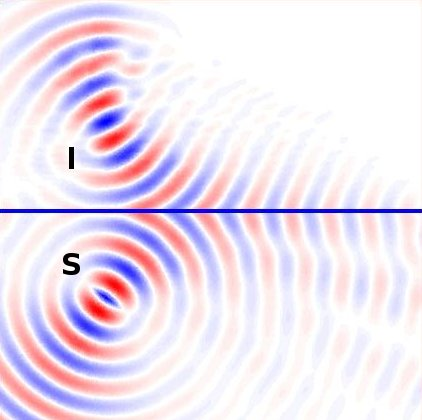
\includegraphics[height=6cm]{pics/nim_lens}
  \end{center}
  \caption{Negative refraction and perfect lens effect. The lower half
    plane is a PIM and the upper half plane is a NIM, with the same
    absolute value of the refractive index. Perfect self focusing is
    achieved. ``S'' stands for ``Source'', ``I'' for ``Image''. We can
    see some power reflected by the interface, at a frequency for
    which PIM and NIM are not matched.}
  \label{fig:nim_lens}
\end{figure}

The simulation has been carried out with a dispersive version of our
algorithm. Kramers-Konig relations impose that a negative index
material must be dispersive in order to not violate causality
\cite{jackson_classical}. Besides, even if only monofrequency sources
are present in the simulation, at regime, in the transient time, when
sources are ``switched on'', many frequencies are present: naively
setting negative $\epsilon$ and $\mu$ into the algorithm makes it
unstable. A fully dispersive algorithm must be employed.

We have implemented dispersive materials for the two-dimensional
time-domain algorithm, with barycentric dual grids (see
\secref{sec:barycentric}). The model chosen is the one described in
\cite{taflove_computational} of Drude media.

The algorithm has been employed to study more in detail the negative
refraction phenomenon, with particular attention to a time-limited,
i.e. broadband, input field. Each frequency in the input spectrum will
see a different refractive index for the NIM, due to its dispersive
nature, some will be negatively refracted, some positively and some
totally reflected \cite{bolla_energy}. The spatial spreading of
frequencies due to this phenomenon has been studied to be used as an
optical multiplexer/demultiplexer \cite{wu_superprism}.

\index{Negative index material|)}










%% \section{FDTD}\label{sec:fdtd}
%% caso particolare di questo schema: griglia ortogonale strutturata, ma
%% pur sempre staggered uncolocated

%% \subsection{Setting Up the Sources}
%% Equivalence Theorem

%% \subsection{parallelization with OPENMP \cite{openmp}}

%% \section{Order-N}
%% Andrej's method: griglia ortogonale strutturata, ma unstaggered
%% colocated (forward/backward differences)

%% \section{FETD}
%% griglia non ortogonale non strutturata, ma staggered e colocated

%% stability condition \cite{marrone_computational}
%% \begin{equation}
%%   \deltat \le \min \left[
%%     \min_k \left( \frac{1}{c_k} \sqrt{
%%       \frac{2 v_k}{\sum_\beta \Abs{d_{k_\beta}}
%%       \frac{s_\beta}{\Dual{\ell}_\beta}}
%%     } \right),
%%     \min_h \left( \frac{1}{c_h} \sqrt{
%%       \frac{2 \Dual{v}_h}{\sum_\alpha \Abs{\Dual{d}_{h_\alpha}}
%%       \frac{\Dual{s}_\alpha}{\ell_\alpha}}
%%     } \right)
%%     \right]
%% \end{equation}  

%% \subsection{PML}
%% PML for unstructured grids in the time domain

%% \subsection{Setting Up the Sources}
%% Equivalence Theorem

%% \section{Benchmarks -- 7 Problems}
%% blah

%% \OKKIO{FDTD dispersive: drude medium -- taflove}
%% \OKKIO{articolo}

